\chapter{Lecture 26 - Laplace's Equation}
\label{ch:lec26}
\section{Objectives}
\begin{itemize}
\item Solve a boundary value problem based on Laplace's equation representing steady-state temperature in a rectangular domain.
\item Show how to use the superposition principle to solve Laplace's equation with multiple non-homogeneous boundary conditions.
\end{itemize}
\setcounter{lstannotation}{0} %hack to try and re-set annotation counter.

\section{Laplace Equation Example}
Consider the system depicted in Figure \ref{fig:lec26-fig1} and described by the following boundary value problem based on Laplace's equation.
\begin{marginfigure}
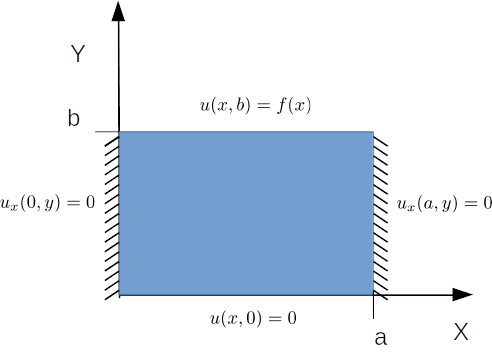
\includegraphics{lec26_fig1.png}
\caption{Schematic of example Laplace's equation problem.}
\label{fig:lec26-fig1}
\end{marginfigure}
\begin{table}[h]
\begin{tabular}{l l}
$\substack{\text{Governing} \\\text{Equation}}: $& $\frac{\partial^2 u}{\partial x^2} + \frac{\partial^2 u}{\partial y^2} = 0, \ \ 0<x<a, \ \ 0<y<b $\\
& \\
$\substack{\text{Boundary} \\ \text{Conditions}}: $ & $\substack{u(x,0)=0  \ \ \ \ \ \ u_x(0,y) = 0 \\ \\ u(x,b) = f(x) \ \ u_x(a,y) = 0}$ 
\end{tabular}
\end{table} 
\noindent We will find the solution to this boundary value problem using separation of variables.

\vspace{0.25cm}

\noindent\textbf{Step \#1:} Assume a product solution.
\begin{equation*}
u(x,y) = F(x)G(y)
\end{equation*}

\vspace{0.25cm}

\noindent\textbf{Step \#2:} Insert proposed solution into the governing equation.

\begin{align*}
\frac{\partial^2}{\partial x^2}\left[F(x)G(y)\right] + \frac{\partial^2}{\partial y^2}\left[F(x)G(y)\right] &= 0 \\
F_{xx}G + FG_{yy} &= 0
\end{align*}

\vspace{4.5cm}

\noindent\textbf{Step \#3:} Separate variables by dividing by $F(x)G(y)$:\marginnote{Once again we assume that neither $F(x)$ nor $G(y)$ are identically equal to zero throughout the domain, therefore it is mathematically acceptable for them to appear in the denominator.}
\begin{align*}
\frac{F_{xx}G}{FG} + \frac{FG_{yy}}{FG} &= 0 \\
\frac{F_{xx}}{F} + \frac{G_{yy}}{G} &= 0 \\
\frac{F_{xx}}{F} = -\frac{G_{yy}}{G} &= -\lambda \\
F_{xx}+\lambda F &= 0 \\
G_{yy}-\lambda G &= 0
\end{align*}
This gives us two separated boundary value problems to solve.

\vspace{0.5cm}

\noindent\textbf{Step \#4:} Apply boundary conditions to determine non-trivial product solution(s).
\begin{marginfigure}
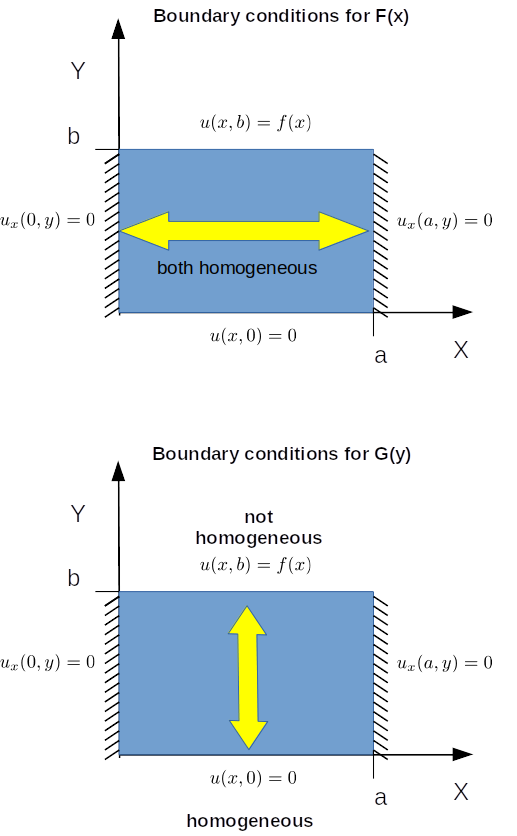
\includegraphics{lec26_bcs.png}
\caption{Pairs of boundary conditions for Laplace's equation.}
\label{fig:lec26-bcs}
\end{marginfigure}

\vspace{0.1cm}

\noindent In order to determine allowable values for $\lambda$, we find solutions to the separated boundary value problem that has \emph{all homogeneous boundary conditions.}\sidenote{If neither separated boundary value problem has all homogeneous boundary conditions, you will need to solve the problem in multiple phases and use the superposition principle to obtain an answer.  This is discussed in the last section of this lecture.}  So we will examine $F_{xx} + \lambda F = 0$.  As usual, we will have to check for all possible values of $\lambda$.

\vspace{0.1cm}

\noindent\underline{$\lambda = 0$}:

\begin{align*}
F_{xx} &= 0 \\
F(x) &= c_1x + c_2 \\
\Rightarrow F_{x} &= c_1 \\
F_x(0) = c_1 &= 0 \\ 
F_{x}(a) &= 0 \ \text{ (satisfied)}
\end{align*}

\vspace{0.1cm}

\noindent We see that, while $c_1$ must be zero, $F(x)=c_2$ satisfies both boundary conditions for any value of $c_2$.  Thus $\lambda = 0$ is an acceptable eigenvalue and the corresponding eigenfunction is a constant.

\vspace{0.1cm}

\noindent\underline{$\lambda < 0$}: To ensure $\lambda$ is negative we will set $\lambda = -\alpha^2, \ \alpha>0$.
\marginnote[1.5cm]{Since the domain is bounded between $0<x<a$, we will use the $\cosh{}$ and $\sinh{}$ form of the solution.}
\begin{align*}
&F_{xx} - \alpha^2 F = 0 \\
&F(x) = c_1 \cosh{\alpha x} + c_2 \sinh{\alpha x} \\
&F_x(x) = \alpha c_1 \sinh{\alpha x} + \alpha c_2 \cosh{\alpha x} \\
&F_x(0) = \alpha c_1 (0) + \alpha c_2 (1) = 0 \\
&\Rightarrow c_2 = 0 \\
&F_x(a) = \alpha c_1 \sinh{a \alpha} = 0\\
&\Rightarrow c_1 = 0
\end{align*}
\marginnote[-1.5cm]{For this last two lines, recall that $\sinh{x}$ is positive for all $x>0$.}
Therefore only the trivial solution $F(x)=0$ satisfies the separated equation and boundary conditions if $\lambda < 0$.

\vspace{0.5cm}

\noindent\underline{$\lambda > 0$}: To insure $\lambda$ is positive we will set $\lambda = \alpha^2, \ \alpha>0$.

\begin{align*}
&F_{xx}+\alpha^2 F = 0 \\
&F(x) = c_1 \cos{\alpha x} + c_2 \sin{\alpha x} \\
&F_{x}(x) = -\alpha c_1 \sin{\alpha x} + \alpha c_2 \cos{\alpha x} \\
&F_{x}(0) = -\alpha c_1 (0) + \alpha c_2 (1) = 0 \\
&\Rightarrow c_2 = 0 \\
&F_{x}(a) = -\alpha c_1 \sin{\alpha a} = 0
\end{align*}
This last condition, $\sin{\alpha a} = 0$, will be satisfied whenever $\alpha a$ is an integer multiple of $\pi$, therefore the eigenvalues are: $\alpha_n = \sfrac{n \pi}{a}, \ \ n\in \mathcal{Z}^+$.\marginnote[-0.25cm]{Note that we do not include $n=0$ since $\alpha>0$.}  The corresponding eigenfunctions are: $F_n(x) = c_1 \cos{\alpha_n x}$.

\vspace{0.25cm}

\noindent In summary, non-trivial eigenfunctions exist when $\lambda = 0$ and when $\lambda >0$.  We need to find the corresponding solutions to $G(y)$ for these cases.

\vspace{0.1cm}

\noindent\underline{$\lambda = 0$}: 
\begin{align*}
G_{yy} &= 0 \\
G(y) &= c_3y + c_4 \\
G(0) &= c_3(0) + c_4 = 0 \\
\Rightarrow c_4 &= 0
\end{align*} \marginnote[-1.0cm]{Apply the homogeneous boundary condition on $G(y)$.}
So the product solution for the case $\lambda = 0$ is: $F(x)G(y) = c_1 c_3y = c_0y$

\vspace{0.25cm}

\noindent\underline{$\lambda = \alpha_n^2$}, $\ \ \alpha_n = \sfrac{n \pi}{a}$.

\begin{align*}
&G_{yy} - \alpha_n^2 G = 0 \\
&G(y) = c_3 \cosh{\alpha_n y} + c_4 \sinh{\alpha_n y} \\
&G(0) = c_3 (1) + c_4(0) \\
&\Rightarrow c_3 = 0 \\
&\Rightarrow G_n(y) = c_4 \sinh{\alpha_n y}
\end{align*}
Therefore the product solution for the case $\lambda > 0$ is: $F_n(x)G_n(y) = c_n \cos{\alpha_n x} \sinh{\alpha_n y}$.\marginnote{We combine all previous constants for each eigenfunction into $c_n$.}

\vspace{0.25cm}

\noindent The full product solution is, therefore:
\begin{equation*}
u(x,y) = c_0y + \sum\limits_{n=1}^{\infty} c_n \cos{\frac{n \pi x}{a}} \sinh{\frac{n \pi y}{a}}
\end{equation*}

\vspace{3.0cm}

\noindent\textbf{Step \#5:} Apply (remaining) boundary condition to determine unknown coefficients.

\vspace{0.25cm}

\noindent The boundary condition that we have not yet used is the non-homogeneous condition applied at $u(x,b)$.  We must find suitable values for $a_0$ and $a_n, \ n=1,2,3,\dots$ such that:
\begin{equation*}
u(x,b) = a_0b + \sum\limits_{n=1}^{\infty}a_n \cos{\frac{n \pi x}{a}}\sinh{\frac{n \pi b}{a}} = f(x)
\end{equation*}
We will find the coefficients the same way we always have: multiply both sides by an orthogonal function and integrate.  The eigenfunctions identified above comprise our set of orthogonal functions.

\vspace{0.25cm}

\noindent For $n=0$:\marginnote{
Some notes on this process:

\begin{enumerate}
\item The eigenfunctions are solutions to the separated equation for $F(x)$ and they are orthogonal over the range $x \in [0,a]$; that is why the integrals are all from 0 to $a$.  

\item $F_0(x) = 1$ is orthogonal to $F_n(x) =  \cos{\sfrac{n \pi x}{a}}$ so all of the terms in the summation are equal to zero.
\end{enumerate}

}
\begin{align*}
c_0 b (1) \int_{0}^{a} \ dx + \sum\limits_{n=1}^{\infty} a_n \cancelto{0}{\left[\int_0^a (1)\cos{\frac{n \pi x}{a}} \ dx \right]} \sinh{\frac{n \pi b}{a}} &= \int_{0}^a f(x)(1) \ dx \\
c_0 (b) (a) &= \int_0^a f(x) \ dx \\
c_0 &= \frac{1}{ab}\int_0^a f(x) \ dx
\end{align*}

\vspace{0.25cm}

\noindent For $n=1,2,3,\dots$ the process is similar, we will show the calculation explicitly for $n=1$:
\marginnote[1.0cm]{You should confirm that: $\int_0^a \cos{\left(\frac{n \pi x}{a}\right)}^2 \ dx = \frac{a}{2}$.

}
%\begin{fullwidth}
\begin{multline*}
c_0b\cancelto{0}{\int_{0}^{a} \cos{\frac{n \pi x}{a}} \ dx} + c_1\left[\int_0^a \cos{\left(\frac{\pi x}{a}\right)}^2 \ dx \right]\sinh{\frac{\pi b}{a}} + \\ \sum\limits_{n=2}^{\infty} \cancelto{0}{\left[\cos{\frac{n \pi x}{a}}\cos{\frac{ \pi x}{a}} \ dx \right]}\sinh{\frac{n \pi b}{a}} = \int_0^a f(x) \cos{\frac{\pi x}{a}} \ dx 
\end{multline*}
\begin{align*}
\Rightarrow c_1 \left(\frac{a}{2} \right)\sinh{\frac{\pi b}{a}} &= \int_0^a f(x) \cos{\frac{\pi x}{a}} \ dx \\
c_1 &= \frac{2\int_0^a f(x) \cos{\frac{\pi x}{b}} \ dx}{a \sinh{\frac{\pi b}{a}}}
\end{align*}
%\end{fullwidth}
and, in general:
\begin{equation*}
c_n = \frac{2\int_0^a f(x) \cos{\frac{n \pi x}{b}} \ dx}{a \sinh{\frac{n \pi b}{a}}}
\end{equation*}

\vspace{0.25cm}

\noindent In summary, the solution to this boundary value problem is:
\begin{equation*}
u(x,y) = c_0y + \sum\limits_{n=1}^{\infty} c_n \cos{\frac{n \pi x}{a}} \sinh{\frac{n \pi y}{a}}
\end{equation*}
where
\begin{align*}
c_0 &= \frac{1}{ab}\int_0^a f(x) \ dx \\
c_n &= \frac{2\int_0^a f(x) \cos{\frac{n \pi x}{b}} \ dx}{a \sinh{\frac{n \pi b}{a}}}
\end{align*}

\section{Implementation in MATLAB}

To actually calculate and plot a solution we need to specify values for $a$, $b$, and $f(x)$ as well as choose a finite number of terms to the infinite series solution.  For this example we will set $a=3$, $b=5$, and we will use $N=25$ terms of the infinite series and we will define the type 1 boundary condition at $y=b$ to be:
\begin{equation*}
f(x) = 
\begin{cases}
x^2, & 0 < x < \sfrac{3}{2} \\
\left(\sfrac{3}{2} \right)^2, & \sfrac{3}{2} \le x < 3
\end{cases}
\end{equation*}

\begin{lstlisting}[name=lec26-ex1, style=myMatlab]
clear
clc
close 'all'

%% Set Parameters
a = 5;
b = 3;
N = 15;

f = @(x) ex1(x,a);

%% define the eigenvalues and eigenfunctions
alpha = @(n) n.*pi./a;
F = @(x,n) cos(alpha(n).*x);
G = @(y,n) sinh(alpha(n).*y);

%% Compute coefficients
% compute Ao
co = (1/(a*b))*integral(@(x) f(x),0,a);

% initialize solution
u = @(x,y) co.*y;
for n = 1:N
    % compute An
    cn = (2./(a*G(b,n))).*...
        integral(@(x) f(x).*F(x,n),0,a);
    % update the approximate solution
    u = @(x,y) u(x,y) + cn*F(x,n).*G(y,n);
end
\end{lstlisting}

\vspace{0.2cm}

\noindent Since this is a two-dimensional geometry, a surface plot is appropriate for visualizing the solution.

\marginnote{

\vspace{4.0cm}

\ref{lst:ann26-1-1} Since the string used for the title includes an apostrophe, double-quotes must be used to enclose the string.

}
\begin{lstlisting}[name=lec26-ex1, style=myMatlab]
%% Make discrete spatial coordinate axes
Nx = ceil(100*a);% "ceil" rounds up to next highest integer
Ny = ceil(100*b);
X = linspace(0,a,Nx);
Y = linspace(0,b,Ny);

[XX,YY] = meshgrid(X,Y);

%% Plot the solution in a 2D plot using surf
figure(1)
surf(XX,YY,u(XX,YY),'edgecolor','none');
title("Lecture 26 Laplace's Equation Example",.../*!\annotation{lst:ann26-1-1}!*/
    'fontsize',16,'fontweight','bold');
xlabel('X','fontsize',14,'fontweight','bold');
ylabel('Y','fontsize',14,'fontweight','bold');
zlabel('u(X,Y)','fontsize',14,'fontweight','bold');
set(gca,'fontsize',12,'fontweight','bold');
\end{lstlisting}
We have saved the definition for \lstinline[style=myMatlab]{ex1(x)} until last since, as usual, we have implemented it as a local function and it must come at the end of the script file.

\begin{lstlisting}[name=lec26-ex1,style=myMatlab]
%% Local functions
function y = ex1(x,a)
[m,n] = size(x);
y = nan(m,n);
for i = 1:length(x)
    if(x(i)>= 0) && (x(i)<a/2)
        y(i) = x(i)^2;
    elseif(x(i) >= a/2) && (x(i)<a)
        y(i) = (a/2)^2;
    end
end    
end
\end{lstlisting}
The resulting plot is shown in Figure \ref{fig:lec26-ex1-sol}.  Readers are strongly encouraged to run this script in MATLAB and examine the output carefully and satisfy yourself that it, at a minimum, meets the specified boundary conditions.
\begin{marginfigure}
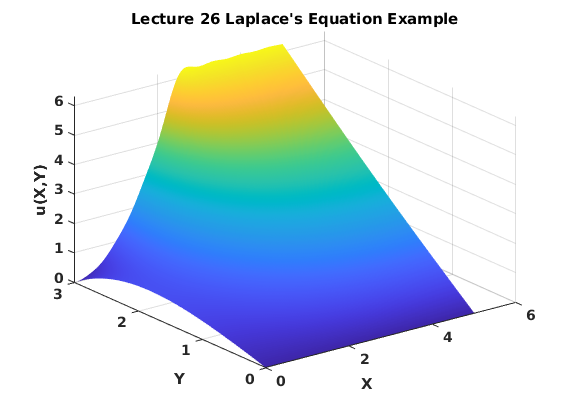
\includegraphics{lec26-ex1-sol.png}
\caption{Surface plot of solution to example problem.}
\label{fig:lec26-ex1-sol}
\end{marginfigure}

\section{Superposition Principle}

In the last example problem, all of the boundary conditions were homogeneous except for along the top edge of the rectangular domain at $y=b$.  We were able to use separation of variables and find a solution because there was one spatial dimension along which \emph{both boundaries were homogeneous.}  Specifically, the boundaries at $x=0$ and $x=a$ had homogeneous type 2 boundary conditions.\marginnote[-1.5cm]{In all of the boundary value problems we have solved so far, this condition has always been met.  In the heat equation and wave equation boundary value problems, there were always homogeneous boundary conditions in the separated boundary value problem for the spatial independent variable $(x)$.  The separated boundary value problem for the temporal independent variable $(t)$ had non-homogeneous boundary (initial) conditions.}   

\begin{marginfigure}
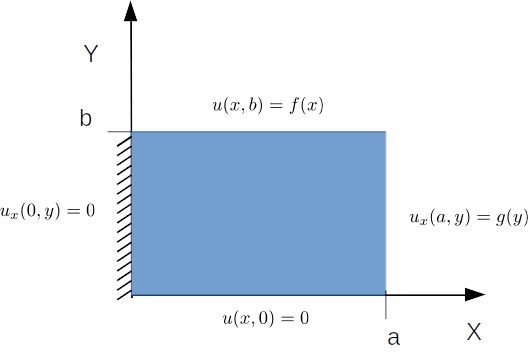
\includegraphics{lec26-ex2-bcs.png}
\caption{Neither spatial dimension has all homogeneous boundary conditions.}
\label{fig:lec26-ex2-bcs}
\end{marginfigure}
What if, instead, we had boundary conditions as depicted by Figure \ref{fig:lec26-ex2-bcs}.  If these were boundary conditions for Laplace's equation, we would carry out separation of variables to derive the two separated boundary value problems just as before.
\begin{align*}
F_{xx}+\lambda F &= 0 \\
G_{yy}-\lambda G &= 0
\end{align*}
Suppose we assumed $\lambda = 0$ and tried to find solutions for $F(x)$, we would get:
\begin{align*}
F(x) &= c_1 x + c_2 \\
F(0) &= c_1 (0) +  c_2 = 0 \\
\Rightarrow c_2 &= 0 \\
F(a) &= c_1(a) = g(y) \ \ \leftarrow \text{  Problem!!}
\end{align*}
Everything is going fine until we have the condition $c_1(a) = g(y)$.  Unless $g(y)$ is a constant: a) no value of $c_1$ will satisfy $g(y)$ for all values of $y \in [0,b]$; and b) there is nothing we can do about it.  We are simply stuck.  The same problem would occur if $\lambda$ were non-zero or if we did the same analysis on $G(y)$.  We need to do something different.


\newthought{What we will do} is this: decompose the problem into two boundary value problems: Problem A and Problem B as is illustrated in Figure \ref{fig:lec26-ex2-bcs-super}.  Each boundary value problem in this decomposition will have one dimension for which there are homogeneous boundary conditions on both boundaries.
\begin{marginfigure}
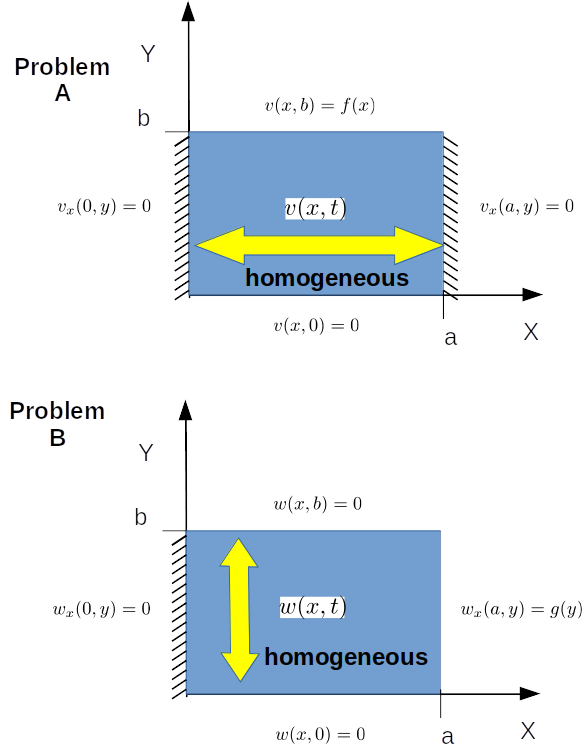
\includegraphics{lec26-ex2-bcs-super.png}
\caption{Superposition of two BVPs each with homogeneous boundary conditions in one dimension.}
\label{fig:lec26-ex2-bcs-super}
\end{marginfigure}
\begin{table}
\begin{tabular}{l l | l}
 & Problem A & Problem B \\ 
 $\substack{\text{Governing} \\ \text{Equation}}$ & $\frac{\partial^2 v}{\partial x^2} + \frac{\partial^2 v}{\partial y^2}=0$ & $\frac{\partial^2 w}{\partial x^2} + \frac{\partial^2 w}{\partial y^2}=0$\\
 & & \\
 $\substack{\text{Boundary}\\\text{Conditions}}$ & $\substack{v_x(0,y) = 0 \ \ v(x,0) = 0\\ v_x(a,y) = 0, \ \ v(x,b)=f(x)}$ & $\substack{w_x(0,y) = 0 \ \ w(x,0) = 0 \\ w_x(a,y) = g(x), \ \ w(x,b) = 0}$
\end{tabular}
\end{table}

\vspace{0.25cm}


\noindent We then solve each boundary value problem to get $v(x,y)$ and $w(x,y)$.  The solution to the original problem is the \emph{superposition} (or just: sum) of the solutions to the sub-problems:
\begin{equation*}
u(x,y) = v(x,y) + w(x,y)
\end{equation*}

\vspace{0.25cm}

\noindent\textbf{Notes:}

\begin{enumerate}
\item This superposition method \emph{requires} that the governing equation and boundary conditions for the boundary value problem all be \underline{linear}.  
\item The method also depends on the fact that the governing equation is \underline{homogeneous}.
\item You should break the problem up into as many sub-problems as is required so that, in each sub-problem, there is one dimension (spatial or temporal) that has homogeneous conditions at all boundaries.
\end{enumerate}
